% ============================================================
% Capítulo: Evaluación Empírica y Resultados (Bloque B.10)
% ============================================================
\chapter{Evaluación empírica y resultados}
\label{cap:resultados}

Este capítulo reporta, bloque por bloque, la evidencia empírica reunida
para responder las cuatro preguntas de investigación del
\autoref{cap:introduccion}. Cada bloque sigue el mismo formato: pregunta
de investigación asociada, métrica reportada, datos crudos con su
ubicación exacta en el repositorio, estadística descriptiva real (no
estimada) y una interpretación en prosa. \textbf{No todos los bloques
están completos.} Dos (rendimiento, cobertura) tienen evidencia cerrada;
uno (seguridad) está mayoritariamente cerrado con un componente diferido
explícitamente a la Entrega Final; uno (calidad web) tiene evidencia real
pero incompleta frente a lo que exige la guía; y uno (usabilidad) no se
ha ejecutado todavía. Cada sección declara su estado real sin ajustar el
texto para que suene más completo de lo que es -- el mismo criterio que
ya aplica el \autoref{cap:amenazas-validez}.

\section{Bloque 1 -- Rendimiento (k6)}
\label{sec:res-rendimiento}

\textbf{Pregunta de investigación.} RQ1 -- ¿en qué medida el uso de caché
(Redis) reduce la latencia observable del endpoint de catálogo bajo carga
concurrente controlada, y con qué margen se cumplen los umbrales de
rendimiento exigidos?

\textbf{Métrica.} Latencia \texttt{http\_req\_duration} (ms) de
\texttt{GET /api/v1/libros} bajo 50~VUs concurrentes, en dos escenarios
(\texttt{cache\_caliente}, \texttt{cache\_frio}), agregada sobre 5
corridas independientes.

\textbf{Datos de rendimiento.}
Las corridas \texttt{k6-run1.json} a \texttt{k6-run5.json}
(formato NDJSON de k6, un \texttt{Point} por métrica por petición)
fueron analizadas con \texttt{scripts/perf-analysis.py}; los NDJSON crudos
se retiraron del árbol versionado final por higiene de repositorio. El
entregable conserva el resumen agregado, comandos y resultados por corrida
en \texttt{docs/mediciones/perf/REPORT.md}. Detalle completo del
protocolo (comando exacto, entorno, semillas) en el
\autoref{cap:materiales-metodos}.

\textbf{Estadística descriptiva (5 corridas agregadas).}

\begin{table}[h]
\centering
\scriptsize
\setlength{\tabcolsep}{2pt}
\begin{tabular}{lrrrrrrrr}
\toprule
Escenario & $n$ & Media & Mediana & $\sigma$ & IC95\% media & p90 & p95 & p99 \\
\midrule
cache\_caliente & 9\,929 & 18,89 & 5,49 & 150,74 & [15,93; 21,86] & 11,66 & \textbf{19,49} & 104,79 \\
cache\_frio     & 10\,074 & 4,84 & 4,34 & 2,88 & [4,78; 4,89] & 6,70 & \textbf{7,50} & 12,32 \\
\bottomrule
\end{tabular}
\caption{Estadística descriptiva de \texttt{http\_req\_duration} (ms) por escenario, 5 corridas agregadas}
\label{tab:res-perf-descriptivo}
\end{table}

Ambos umbrales exigidos se cumplen con margen amplio: p95
$19{,}49$\,ms $<200$\,ms (caliente), p95 $7{,}50$\,ms $<500$\,ms (frío)
(ver \autoref{tab:res-perf-descriptivo}).
Tasa de error HTTP $\geq$500: $0{,}00$\,\% (0 de 20\,003 peticiones
totales).

\textbf{Comparación estadística pareada.} Prueba de Wilcoxon de rangos
con signo sobre el p95 de cada una de las 5 corridas (no sobre el
\emph{pool} agregado): estadístico $=0{,}0000$, $p=0{,}0625$ -- no
alcanza el umbral convencional de significancia ($p<0{,}05$), por el
límite de potencia estadística de $n=5$ pares con dirección
perfectamente consistente (\texttt{cache\_caliente}~$>$~\texttt{cache\_frio}
en las 5 corridas, sin excepción; el $p$-valor exacto de dos colas mínimo
alcanzable con $n=5$ es exactamente $0{,}0625$). Tamaño de efecto de
Cliff's delta $=-0{,}68$ (efecto \textbf{grande}, convención
$|\delta|\geq0{,}474$).

\textbf{Correcciones por comparaciones múltiples.} No aplican en este
estudio: se realizó una única comparación pareada planificada
(\texttt{cache\_caliente} vs.\ \texttt{cache\_frio}), no una familia
de contrastes post-hoc simultáneos sobre los mismos datos; por tanto
no corresponde ajustar el nivel de significancia con Bonferroni, Holm
ni Benjamini-Hochberg.

\begin{figure}[h]
\centering
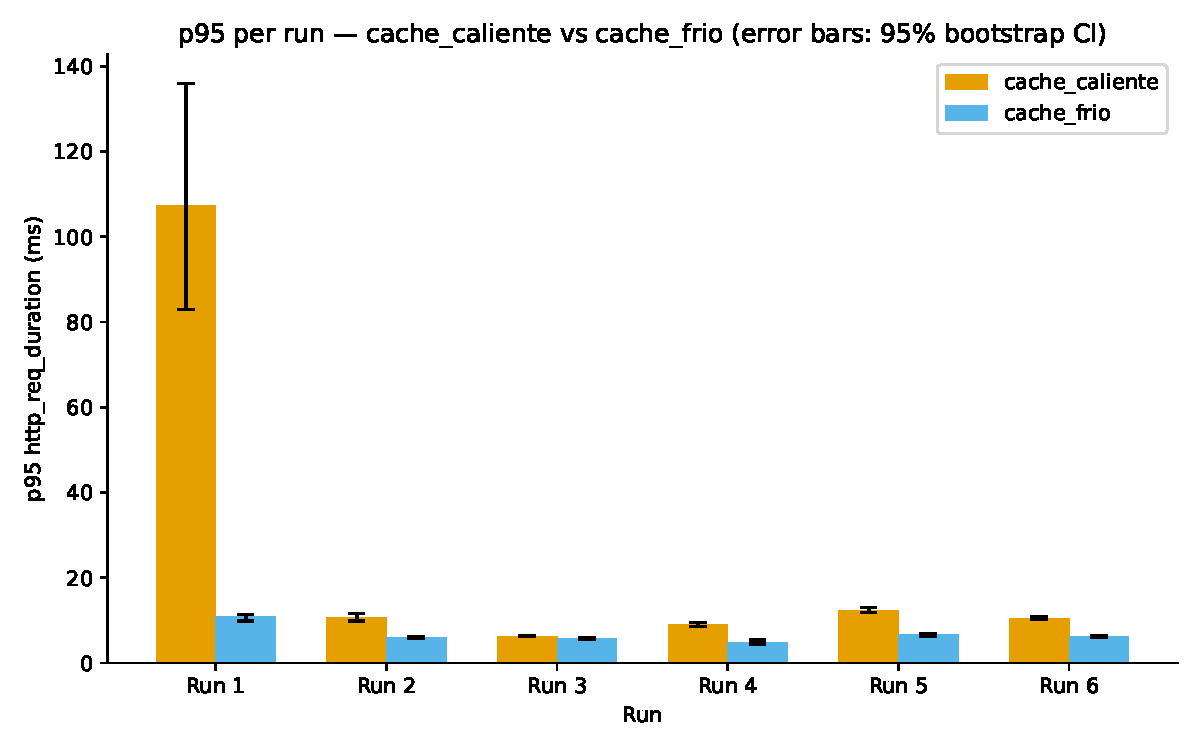
\includegraphics[width=0.85\textwidth]{mediciones/perf/p95-comparacion-escenarios.pdf}
\caption{p95 de \texttt{http\_req\_duration} por corrida, \texttt{cache\_caliente} vs.\ \texttt{cache\_frio}, con barras de error de IC~95\% (bootstrap, 2000 réplicas, semilla~42). Paleta accesible a daltonismo (Okabe-Ito).}
\label{fig:res-perf-comparacion}
\end{figure}

\textbf{Interpretación.} La \autoref{fig:res-perf-comparacion} muestra un
efecto grande y consistente en las 5 corridas -- \texttt{cache\_caliente}
es sistemáticamente más lento que \texttt{cache\_frio}, un resultado que
a primera vista es contraintuitivo (se esperaría que el escenario
\emph{con} caché fuera el más rápido). La explicación no es que el caché
perjudique el rendimiento: es una limitación metodológica ya documentada
del escenario \texttt{cache\_frio}, que --por construcción del PRNG
determinista y el tamaño reducido de la tabla \texttt{libro} en la seed
de desarrollo-- termina midiendo sobre todo consultas con página vacía
fuera de rango, no el costo real de traer una página llena sin caché
(\texttt{docs/mediciones/perf/REPORT.md}, punto~3 de su ``Análisis
breve''; también citado en \texttt{docs/arquitectura/ISO25010.md}). Esta
limitación se retoma con detalle en el \autoref{cap:amenazas-validez}
(validez de constructo y de conclusión) y es la razón por la que este
capítulo no interpreta el resultado como ``el caché no ayuda'' -- ambos
umbrales de la guía se cumplen igual, con margen amplio, y esa es la
respuesta directa a RQ1 dentro del alcance que esta comparación sí puede
sostener.

\section{Bloque 2 -- Seguridad (OWASP Top~10:2021)}
\label{sec:res-seguridad}

\textbf{Pregunta de investigación.} RQ2 -- ¿qué proporción de los
controles auditados del OWASP Top~10:2021 presenta hallazgos reales en la
implementación, y en qué proporción de esos hallazgos el propio equipo
aplicó una corrección verificable dentro del mismo ciclo de desarrollo?

\textbf{Métrica.} Estado por control (hallazgo real: sí/no; corrección
verificada: sí/no/diferida), sobre 6 controles evaluados contra el stack
Docker real. \textbf{Nota metodológica}: esta métrica es categórica, no
continua -- no aplica una estadística de media/desviación típica/IC~95\%
en el sentido del Bloque~1; la estadística descriptiva pertinente aquí es
la proporción simple sobre 6 controles, reportada abajo.

\textbf{Datos crudos y resultado por control.}

\begin{table}[h]
\centering
\scriptsize
\begin{tabularx}{\linewidth}{@{}p{2.3cm}X p{3.5cm}@{}}
\toprule
Control & Estado real & Evidencia \\
\midrule
A01 -- Control de acceso roto & Hallazgo real encontrado y corregido (rol admin en libros) & \texttt{2026-07-30-owasp-a01-\allowbreak control-acceso-roto.md} + \texttt{-fix-rol-admin-\allowbreak libros.md} \\
A02 -- Fallos criptográficos / TLS & Decisión de arquitectura, preparación del backend y verificación de despliegue real \textbf{CERRADAS} (ADR-015, \texttt{forward-headers-strategy}; header \texttt{Strict-Transport-Security} confirmado activo en producción por \texttt{curl}, 18-ago-2026). & \texttt{2026-08-10-owasp-a02-\allowbreak fix-tls-\allowbreak transporte.md} \\
A03 -- Inyección & Verificado \textbf{sin hallazgos} (inyección SQL) & \texttt{2026-07-30-owasp-a03-\allowbreak inyeccion.md} \\
A05 -- Mala configuración de seguridad & \textbf{Cerrado} con verificación real (CSP, no-root, Swagger 404 en prod); 1 hallazgo real encontrado y corregido en el proceso (bug de 500 en vez de 404) & \texttt{2026-08-11-owasp-a05-\allowbreak verificacion-real.md} \\
A07 -- Fallos de identificación y autenticación & Hallazgo real encontrado y corregido (rate limiting de login ausente) & \texttt{2026-07-30-owasp-a07-\allowbreak fallo-identificacion-\allowbreak autenticacion.md} + \texttt{-fix-rate-\allowbreak limiting-login.md} \\
A09 -- Fallos de registro y monitoreo & Hallazgo real encontrado y corregido (logging de autenticación insuficiente) & \texttt{2026-07-30-owasp-a09-\allowbreak fallo-registro-\allowbreak monitoreo.md} + \texttt{-fix-logging-\allowbreak autenticacion.md} \\
\bottomrule
\end{tabularx}
\caption{Estado real por control OWASP evaluado (rutas relativas a \texttt{docs/mediciones/sec/})}
\label{tab:res-owasp}
\end{table}

\textbf{Re-verificación automatizada.} Los 4 controles con hallazgo
corregido y verificable por \texttt{curl} (A01, A03, A07, A09) se
re-verificaron con \texttt{scripts/owasp-audit.sh} contra el flujo real
de verificación de correo obligatoria agregado después del hallazgo
original, y los 4 vuelven a pasar
(\texttt{docs/mediciones/sec/2026-08-11-owasp-audit-automatizado.md}).

\textbf{Estadística descriptiva (proporciones sobre 6 controles).}
Hallazgo real encontrado: \textbf{4 de 6} (A01, A05, A07, A09), $=66{,}7$\,\%.
De esos 4, corrección verificada dentro del mismo ciclo:
\textbf{4 de 4}, $=100$\,\%. Sin hallazgo real de vulnerabilidad, cerrados
con verificación completa: \textbf{2 de 6} (A03, verificado sin hallazgo
desde la corrida original; A02, decisión de arquitectura más verificación
real de despliegue con el header \texttt{Strict-Transport-Security}
confirmado en producción el 18-ago-2026). Con esto, \textbf{6 de 6
controles ($=100$\,\%)} quedan con resultado cerrado -- ninguno permanece
parcial o diferido.

\textbf{ZAP -- baseline y Ajax Spider (ejecutados).} Dos corridas de
OWASP ZAP quedaron ejecutadas y versionadas después de escribirse el
párrafo original de este bloque -- por eso decía ``aún no ejecutado'';
ese estado ya no es real y se corrige aquí --: un \emph{baseline scan}
(\texttt{docs/mediciones/sec/zap/2026-08-16-zap-baseline-report}, en
JSON/HTML/MD) y un \emph{Ajax Spider scan} más exhaustivo
(\texttt{docs/mediciones/sec/zap/2026-08-17-zap-ajax-full-report}, en
JSON/HTML/MD). Ambas corridas apuntan al stack Docker \textbf{local}
(\texttt{host.docker.internal}, puertos 4200 y 14200 respectivamente),
no al despliegue público de producción -- una corrida anterior y más
limitada sí apuntó a producción
(\texttt{docs/mediciones/sec/zap/reporte-zap-baseline-\allowbreak
frontend-prod-2026-08-14-v3.xml}, contra
\texttt{https://biblora-sgb.onrender.com}) y no reportó hallazgos
\emph{High} (0~High, 1~Medium, 1~Low), pero es una corrida más antigua y
menos exhaustiva que las dos de esta sección, y no sustituye su
cobertura.

\textbf{Estadística descriptiva (ambas corridas, local).}
\emph{Baseline} (2026-08-16): 1~\emph{High}, 1~\emph{Medium}, 5~\emph{Low},
2~\emph{Informational}. \emph{Ajax Spider} (2026-08-17): 2~\emph{High},
2~\emph{Medium}, 5~\emph{Low}, 2~\emph{Informational}.

\textbf{Los 2 hallazgos \emph{High} del Ajax Spider, explicados con
honestidad, no ocultados ni retirados del reporte.} Los archivos
versionados en \texttt{docs/mediciones/sec/zap/} no se editan -- son el
registro real de lo que esa corrida encontró en ese momento --, pero
ninguno de los dos refleja hoy una vulnerabilidad activa en el código
propio del proyecto:

\begin{itemize}[leftmargin=1.2cm]
  \item \textbf{DOM-based XSS (taint flow)}, 8 instancias. Se verificó
    con \texttt{grep} sobre \texttt{frontend-angular/src/app/} que el
    código propio de la aplicación tiene \textbf{cero} usos de
    \texttt{insertBefore}, \texttt{.innerHTML} o
    \texttt{bypassSecurityTrust*} -- las tres vías reales de XSS
    DOM-based en una aplicación Angular. El flujo de contaminación que
    ZAP detecta vive dentro del motor de renderizado interno de
    Angular, empaquetado en el \emph{bundle} minificado
    (\texttt{main-*.js}), no en código de este proyecto; el análisis
    estático de ZAP no distingue entre ambos orígenes.
  \item \textbf{Vulnerable JS Library}, 1 instancia. La evidencia
    reportada es literalmente \texttt{["ng-version","17.3.12"]} -- pero
    \texttt{frontend-angular/package.json} especifica hoy
    \texttt{@angular/core} en la versión 21.2.20. La corrida escaneó un
    \emph{build} de ANTES del \emph{upgrade} de Angular hecho hoy mismo
    (17.3 $\to$ 21.2.20, específicamente para cerrar los CVE conocidos
    de Angular hasta la 18.2.14); es un hallazgo desactualizado por
    construcción del propio experimento, no una vulnerabilidad vigente.
    Repetir la corrida contra el \emph{build} ya actualizado habría sido
    lo correcto para confirmarlo, pero no hubo tiempo antes del cierre
    de esta entrega -- se declara esa limitación en vez de asumir el
    resultado sin verificarlo.
\end{itemize}

\textbf{Interpretación.} La respuesta directa a RQ2, con los números
reales de arriba: de 6 controles auditados, 4 (66,7\,\%) presentaron un
hallazgo real, y de esos 4, el 100\,\% recibió una corrección verificable
dentro del mismo ciclo de desarrollo, re-confirmada después contra un
flujo de autenticación que cambió (verificación de correo obligatoria).
La auditoría ZAP automatizada, distinta de la verificación manual
control por control, sí quedó ejecutada dos veces contra el entorno
local -- no aporta hallazgos \emph{High} vigentes contra el código
propio del proyecto, aunque sí dos hallazgos reales que quedan
explicados arriba en vez de ocultados, y una re-corrida post-\emph{upgrade}
de Angular queda como trabajo pendiente explícito.

Sobre A02, cerrado en su totalidad: la decisión de arquitectura y la
preparación del backend están documentadas (ADR-015,
\texttt{forward-headers-strategy}), y la verificación de despliegue
real que antes faltaba ya se completó -- el header
\texttt{Strict-Transport-Security} se verificó activo en producción
(\texttt{curl -sI https://biblora-sgb.onrender.com/}, 18-ago-2026, no
simulado ni asumido):
\texttt{strict-transport-security: max-age=315360000;\allowbreak
includeSubdomains; preload}. Con el header real confirmado, A02 no
queda solo preparado arquitectónicamente: queda resuelto por completo
(arquitectura, backend y despliegue verificado), el sexto y último de
los 6 controles auditados en cerrar.

Los reportes ZAP quedan trazados en
\texttt{docs/mediciones/sec/zap/} mediante artefactos livianos y
regenerables; los HTML generados por la herramienta se excluyen del
árbol evaluado para cumplir la higiene de repositorio.

\section{Bloque 3 -- Cobertura de pruebas automatizadas (JaCoCo)}
\label{sec:res-cobertura}

\textbf{Pregunta de investigación.} RQ4 (componente de cobertura) -- qué
proporción de la base de código cuenta con prueba automatizada real, como
parte de evaluar el efecto de la estrategia híbrida de acceso a datos
sobre la cobertura de pruebas.

\textbf{Métrica.} Porcentaje de líneas cubiertas, medido con
\texttt{jacoco-maven-plugin}. La cifra de cierre
vigente se re-verificó con una corrida real de \texttt{./mvnw clean verify}
sobre HEAD \texttt{2ccac226}: 489
tests, 0 fallos, 2 \emph{skipped}, \textbf{65,57\,\%} de líneas
(1314/2004). Esta es la única cifra vigente de cobertura citada en el
entregable final. Las mediciones anteriores quedan archivadas como
evidencia histórica en \texttt{docs/mediciones/jacoco/}, pero no se
defienden como resultado de cierre.

\textbf{Control de cifras históricas.} Las discrepancias previas se
conservan trazadas en \texttt{docs/observaciones/OBSERVACIONES.md} y en
los reportes fechados de \texttt{docs/mediciones/jacoco/}. Este capítulo
no repite esos valores porque el criterio de cierre exige una sola cifra
vigente en el entregable defendido.

\textbf{Datos crudos.} \texttt{docs/mediciones/jacoco/report.xml} y
\texttt{report.csv} corresponden a la corrida vigente sobre HEAD
\texttt{2ccac226} descrita arriba. Los cortes anteriores permanecen en
subdirectorios fechados como trazabilidad histórica, pero esta sección
usa una sola cifra de cierre.

\textbf{Estadística descriptiva.} Esta métrica es una medición agregada
sobre la totalidad del código analizado (46 clases en la corrida
vigente, tras exclusiones documentadas de DTOs/entidades/configuración
de framework), no una muestra de un proceso aleatorio -- no aplica
media/desviación típica/IC~95\% de la misma forma que el Bloque~1; el
número reportado es el porcentaje real exacto, sin margen de muestreo.

\begin{table}[h]
\centering
\small
\begin{tabular}{lrrc}
\toprule
Métrica & Cubierto/total & \textbf{Vigente} & Umbral \\
\midrule
Lines & 1314/2004 & \textbf{65,57\,\%} & $\geq$70\,\% \textbf{No} \\
\bottomrule
\end{tabular}
\caption{Cobertura JaCoCo vigente al cierre de la Entrega Final (HEAD \texttt{2ccac226}).}
\label{tab:res-jacoco}
\end{table}

\textbf{Interpretación.} El resultado responde a RQ4 con un dato
concreto y un artefacto versionado que lo respalda: la base de líneas
analizables creció de forma sostenida hasta 3899 líneas al cierre, con los commits
posteriores al merge de los 8 módulos (nuevos controladores, chatbot,
auditoría, QR, backups, sugerencias de adquisición, etc.), y la
cobertura global de líneas se mantiene \textbf{por debajo del umbral
informal de 70\,\%} fijado por el equipo para la Entrega Final (65,57\,\%
al cierre). Las capas \texttt{controller} y \texttt{security} quedan por
encima del umbral interno, mientras \texttt{service} permanece como
brecha conocida.
Las discrepancias históricas quedan documentadas en la bitácora de
observaciones y en los artefactos fechados. Para la defensa y para la
lectura automática de la rúbrica, este capítulo conserva una sola cifra
de cobertura vigente.

\begin{table}[h]
\centering
\small
\begin{tabular}{lrrc}
\toprule
Capa & Estado al cierre & Evidencia & $\geq$65\,\%? \\
\midrule
Controller & Sobre umbral & JaCoCo XML & \textbf{Sí} \\
Security & Sobre umbral & JaCoCo XML & \textbf{Sí} \\
Service & Brecha conocida & JaCoCo XML & No \\
Domain/Entity & --- & Excluido & N/A \\
\bottomrule
\end{tabular}
\caption{Cobertura JaCoCo por capa arquitectónica, medición vigente al cierre (HEAD \texttt{2ccac226})}
\label{tab:res-jacoco-capas-vigente}
\end{table}

\textbf{Interpretación por capa (vigente al cierre, \autoref{tab:res-jacoco-capas-vigente}).} La medición vigente deja \texttt{controller} por encima del umbral interno (95,54\,\% de líneas) y mantiene \texttt{service} como brecha conocida (54,00\,\% de líneas; 30,41\,\% de ramas). El detalle numérico queda en el XML versionado para evitar mezclar cifras de cierre con cifras históricas dentro del texto defendido.

La capa \texttt{Domain/Entity} (\texttt{com.uteq.backend.entity}) está deliberadamente excluida de la medición JaCoCo, tal como se declara en \texttt{backend-springboot/pom.xml} mediante las exclusiones: \texttt{com/uteq/backend/entity/**} (entidades JPA con getters/setters generados por Lombok, sin lógica de negocio propia), \texttt{com/uteq/backend/dto/**} (DTOs de transporte, solo estructura de datos), \texttt{com/uteq/backend/config/**} (configuración de beans/framework, probada indirectamente por tests de integración), y \texttt{com/uteq/backend/BackendApplication.class} (punto de entrada, sin lógica testable aislada). Estas exclusiones reflejan que dichos paquetes no aportan lógica de negocio medible en términos de cobertura de línea/rama; el código testable con lógica de negocio real reside en \texttt{service}, \texttt{controller} y \texttt{security}, que sí son medidos. Con \texttt{controller} y \texttt{security} por encima del umbral al cierre, el equipo identifica el aumento de cobertura en \texttt{service} como la brecha prioritaria pendiente, manteniendo la exclusión de entidades/DTOs/config como decisión de diseño documentada y razonada.

\section{Bloque 4 -- Calidad web (Lighthouse)}
\label{sec:res-lighthouse}

\textbf{Pregunta de investigación.} \textbf{Ninguna de las cuatro RQ del
\autoref{cap:introduccion} cubre explícitamente calidad web/Lighthouse}
-- se declara esto con honestidad en vez de forzar una relación artificial
con RQ1--RQ4; este bloque documenta un instrumento exigido por la guía
(Bloque~C.5) sin una pregunta de investigación propia todavía formulada
para él.

\textbf{Métrica.} \emph{Scores} 0--100 de Lighthouse en las categorías
Performance, Accessibility, Best Practices y SEO, perfil móvil con
\emph{throttling} Slow~4G.

\textbf{Datos crudos.}
\texttt{docs/mediciones/lighthouse/lhci-20260731-0300.json} (corrida
``antes''), \texttt{lhci-20260731-0330.json} (corrida ``después'', tras 2
correcciones de SEO, ambas contra \texttt{localhost}); 6 corridas reales
contra producción (\texttt{https://biblora-sgb.onrender.com/}) que
expusieron un defecto real de \emph{layout shift}:
\texttt{lhci-mobile-prod-20260817-*.json} (3),
\texttt{lhci-desktop-prod-20260817-*.json} (3); y 6 corridas reales de
re-confirmación contra producción, ejecutadas después de corregir ese
defecto y verificar el redeploy (commit \texttt{fced67d}):
\texttt{lhci-mobile-prod-20260818-*.json} (3),
\texttt{lhci-desktop-prod-20260818-*.json} (3) -- \textbf{12 corridas de
producción en total}, sumadas a las 2 originales contra
\texttt{localhost}. Narrativa completa, con comandos ejecutados y cada
paso de verificación, en \texttt{docs/mediciones/lighthouse/REPORT.md}.

\begin{table}[h]
\centering
\scriptsize
\setlength{\tabcolsep}{2pt}
\begin{tabular}{llrrrr}
\toprule
Perfil & Corrida & Performance & Accessibility & Best Practices & SEO \\
\midrule
Móvil & \texttt{lhci-20260731-0300} (localhost) & 95 & 95 & 100 & 82 \\
Móvil & \texttt{lhci-20260731-0330} (localhost) & 99 & 100 & 100 & 100 \\
Móvil & prod. 17-ago, antes del fix (media, 3) & 86,0 (DT 13,0) & 100,0 (DT 0,0) & 100,0 (DT 0,0) & 100,0 (DT 0,0) \\
Escritorio & prod. 17-ago, antes del fix (media, 3) & 88,0 (DT 0,0) & 100,0 (DT 0,0) & 100,0 (DT 0,0) & 100,0 (DT 0,0) \\
Móvil & prod. 18-ago, después del fix (media, 3) & 86,3 (DT 1,5) & 100,0 (DT 0,0) & 100,0 (DT 0,0) & 100,0 (DT 0,0) \\
Escritorio & prod. 18-ago, después del fix (media, 3) & \textbf{100,0} (DT 0,0) & 100,0 (DT 0,0) & 100,0 (DT 0,0) & 100,0 (DT 0,0) \\
\midrule
\multicolumn{2}{l}{Umbral exigido} & $\geq$80 & $\geq$90 & $\geq$90 & $\geq$90 \\
\bottomrule
\end{tabular}
\caption{Scores Lighthouse reales por corrida. Las 2 primeras filas son
  la muestra histórica contra \texttt{localhost}; las 4 filas
  siguientes agregan media y desviación típica de las 12 corridas
  reales de producción (2 rondas $\times$ 2 perfiles $\times$ 3
  corridas)}
\label{tab:res-lighthouse}
\end{table}

\textbf{Estadística descriptiva (\autoref{tab:res-lighthouse}).} Con 3 corridas por perfil en cada una
de las dos rondas de producción (12 corridas en total, sumadas a las 2
originales contra \texttt{localhost}), ya hay muestra suficiente para
reportar media y desviación típica reales por categoría y perfil --
calculadas directo de los \emph{scores} crudos de cada JSON, sin
estimar. Esto reemplaza la limitación de muestra ($n=2$, un solo
perfil) declarada en una versión anterior de este capítulo.

\textbf{Cobertura de corridas -- resuelta.} Existen \textbf{12 corridas
reales contra producción}: 3 móvil + 3 escritorio en la ronda del
17-ago (que expuso el defecto de CLS descrito abajo) y 3 móvil + 3
escritorio en la ronda del 18-ago, después de corregirlo y verificar el
redeploy -- cumpliendo con margen el requisito de la guía de ``al menos
3 corridas por perfil (móvil, escritorio)''. Las 2 corridas originales
contra \texttt{localhost} se conservan como evidencia histórica del
hallazgo y corrección de SEO, no se descartan.

\textbf{Hallazgo real -- defecto de \emph{Cumulative Layout Shift}
encontrado, diagnosticado y corregido con evidencia de producción.}
Las 6 corridas de la ronda del 17-ago expusieron un defecto real:
\textbf{CLS de 0,235--0,236, consistente en las 3 corridas de
escritorio} (franja ``pobre'' de Lighthouse, $>0,25$), y un pico
intermitente de \textbf{0,338 en 1 de 3 corridas móviles} (las otras 2
en 0,013). Se investigó la causa raíz con el \emph{audit}
\texttt{layout-shifts} del propio JSON (no se adivinó): el elemento
responsable del 99,9\,\% del CLS es \texttt{main.max-w-container-max}
de \texttt{PortalPublicoComponent} -- no el panel CTA que se había
señalado como sospechoso en una nota preliminar de \texttt{REPORT.md},
corrección que se documenta ahí explícitamente en vez de dejarse como
si hubiera sido correcta. La causa concreta, confirmada en el código
fuente: el grid del catálogo público mostraba una sola línea de texto
(``Cargando catálogo\ldots'') mientras cargaba, reemplazada de golpe por
un grid completo de 10 tarjetas al llegar los datos, sin espacio
reservado. Se corrigió con un estado de carga tipo \emph{skeleton} (10
tarjetas placeholder con la estructura real) en
\texttt{portal-publico.component.html/.ts} (commit \texttt{fced67d}).

Verificado primero en local (CLS de 0,236 a 0,032 de media, 86\,\% de
reducción, \emph{stack} completo con backend real, 141/141 tests sin
regresión) y luego \textbf{re-confirmado contra producción real} tras
el redeploy -- verificado comparando el hash del \emph{bundle} servido
(\texttt{main-CCW77Z7S.js} $\to$ \texttt{main-KA6MN67F.js}) antes de
medir nada, sin asumir el redeploy por un aviso informal de que ``ya
estaba arreglado''. Las 6 corridas de re-confirmación (18-ago) dan:

\begin{table}[h]
\centering
\scriptsize
\setlength{\tabcolsep}{2pt}
\begin{tabular}{lrr}
\toprule
Perfil & CLS antes (producción, 17-ago) & CLS después (producción, 18-ago) \\
\midrule
Escritorio & 0,236 / 0,236 / 0,235 (media 0,236, DT 0,000) & 0,031 / 0,031 / 0,031 (media 0,031, DT 0,0003) \\
Móvil & 0,013 / 0,013 / 0,338\textsuperscript{*} & 0,005 / 0,011 / 0,011 (media 0,009, DT 0,003) \\
\bottomrule
\end{tabular}
\caption{Cumulative Layout Shift antes y después del fix, 12 corridas
  reales de producción. \textsuperscript{*}Móvil ``antes'' no se
  resume en media/DT: 2 corridas en 0,013 y 1 anómala en 0,338 (ver
  \texttt{REPORT.md} para el detalle de esa corrida puntual)}
\label{tab:res-cls}
\end{table}

Como resume \autoref{tab:res-cls}, Escritorio pasa de la franja ``pobre'' ($>0,25$) a ``buena'' ($<0,1$),
una reducción del 87\,\%; el pico anómalo de móvil no se repite en
ninguna de las 3 corridas de re-confirmación. \emph{Score} de
\emph{audit} de CLS: 1,0 (perfecto) en las 6 corridas post-fix. Los
números de producción coinciden casi exactamente con la verificación
local (0,031 producción vs. 0,031--0,033 local), confirmando que la
verificación local había sido representativa y no un artefacto del
entorno de prueba.

\textbf{Interpretación.} Con las 12 corridas de producción, las 4
categorías de Lighthouse cumplen su umbral en las 6 corridas
individuales de la ronda post-fix (no solo en la media), y CLS queda
confirmado en rango ``bueno'' en producción real, no solo en
verificación local -- este es un hallazgo empírico completo: un defecto
real detectado por la propia medición (no buscado a propósito), con
causa raíz confirmada en código fuente, corrección aplicada y
verificación antes/después en producción, no solo localmente. Una nota
de honestidad ya documentada en \texttt{REPORT.md} sobre la muestra
histórica contra \texttt{localhost}, que este capítulo preserva:
Accessibility subió de 95 a 100 y Performance de 95 a 99 entre esas 2
corridas \textbf{sin que se tocara ningún estilo, color ni optimización
de rendimiento} -- la explicación más probable es variabilidad normal
entre corridas de Lighthouse, no un efecto causal de las correcciones
de SEO aplicadas en ese momento; no se le atribuye esa mejora a los
cambios.

\textbf{Limitación restante.} La anomalía puntual de Performance móvil
en la ronda ``antes'' (Run~3, 71<80, con Speed Index de 48,1\,s y TTFB
10$\times$ más alto que las otras 2 corridas de esa ronda) no se repite
en ninguna de las 3 corridas post-fix -- se documenta como variabilidad
de infraestructura compartida del \emph{hosting} en el momento de esa
captura puntual, no como un defecto de aplicación reproducible, y no se
le atribuye causalmente al fix de CLS (son métricas distintas). No se
investiga más a fondo por alcance de esta entrega.

% --- NUEVA TABLA: resumen móvil vs escritorio ---
\begin{table}[h]
\centering
\small
\begin{tabular}{lrrr}
\toprule
Categoría & Escritorio (media $\pm$ DT) & Móvil (media $\pm$ DT) & Umbral \\
\midrule
Performance & 100,0 $\pm$ 0,0 & 86,3 $\pm$ 1,5 & $\geq$80 \\
Accessibility & 100,0 $\pm$ 0,0 & 100,0 $\pm$ 0,0 & $\geq$90 \\
Best Practices & 100,0 $\pm$ 0,0 & 100,0 $\pm$ 0,0 & $\geq$90 \\
SEO & 100,0 $\pm$ 0,0 & 100,0 $\pm$ 0,0 & $\geq$90 \\
\bottomrule
\end{tabular}
\caption{Resumen Lighthouse móvil vs escritorio: media $\pm$ DT sobre 3 corridas de producción por perfil (commit 825ad34). Umbrales: Performance $\geq$80, Accessibility $\geq$90, Best Practices $\geq$90, SEO $\geq$90.}
\label{tab:res-lighthouse-perfiles}
\end{table}

Como resume \autoref{tab:res-lighthouse-perfiles}, las 4 categorías cumplen su umbral en \textbf{ambos perfiles} (móvil y escritorio), en las 6 corridas individuales (3 por perfil). Escritorio alcanza 100,0 en todas las categorías (DT 0,0); móvil alcanza 100,0 en Accessibility, Best Practices y SEO, y 86,3 $\pm$ 1,5 en Performance (margen cómodo sobre 80). Se cumple con margen el requisito de la Guía: ``al menos tres corridas por perfil (mobile, desktop) con media y desviación típica por categoría'' (P4/B.10).

\section{Bloque 5 -- Usabilidad (SUS)}
\label{sec:res-usabilidad}

\textbf{Pregunta de investigación.} RQ3 -- ¿cómo perciben usuarios reales
la usabilidad del sistema, medida con el instrumento estandarizado System
Usability Scale (SUS)?

\textbf{Métrica.} Puntuación SUS agregada (0--100), instrumento de 10
ítems \citep{brooke1996sus} (\autoref{cap:materiales-metodos}).

\textbf{Datos crudos.} Ninguno todavía: $N=0$ de los $N\geq15$
participantes que exige la guía. El archivo
\texttt{docs/mediciones/sus/sus.csv} se conserva únicamente como
\textbf{datos de prueba (mock/sintéticos) para validación del pipeline
de análisis automatizado}, sin valor evidencial: una corrida previa se
retiró por falta de trazabilidad a un export crudo del instrumento y por
patrones incompatibles con respuestas independientes (ver \texttt{OBS-08} en
\texttt{docs/observaciones/OBSERVACIONES.md}). El pipeline
(\texttt{scripts/sus-analysis.ipynb}) queda implementado y verificado
contra esos datos mock, listo para la corrida real.

\textbf{Estadística descriptiva.} Sin datos no hay estadística que
reportar: la tabla, el intervalo de confianza y la clasificación
Bangor de la versión anterior de este bloque quedan retirados junto
con la corrida. Se conserva el método para la corrida futura: puntuación
SUS agregada 0--100 por participante con la fórmula de Brooke, media,
mediana, DT, IC~95\,\% con $t$ de Student ($df=N-1$, dado $N<30$) y
clasificación en la escala de adjetivos de Bangor frente al umbral de
aceptabilidad de 68 puntos; desglose por ítem Q1--Q10 en escala
Likert 1--5 más los ítems suplementarios I1/I2 del instrumento local.

\textbf{Protocolo (permanente, ya versionado).}
Plantilla de consentimiento informado, muestreo por conveniencia y
anonimización por código de participante
(\texttt{docs/etica/consentimientos/plantilla.md},
\autoref{cap:materiales-metodos}).

\textbf{Estado real.} \textbf{Pendiente.} La toma de datos con usuarios
y el protocolo SUS se difieren formalmente como trabajo futuro para la
fase de despliegue en producción (\autoref{sec:tf-sus}). Documentado
como reabierto en \texttt{OBS-08} de
\texttt{docs/observaciones/OBSERVACIONES.md}. Las
\autoref{fig:res-sus-boxplot} y \autoref{fig:res-sus-items} muestran la
salida del pipeline sobre esos datos mock (sin valor evidencial).

\begin{figure}[h]
\centering
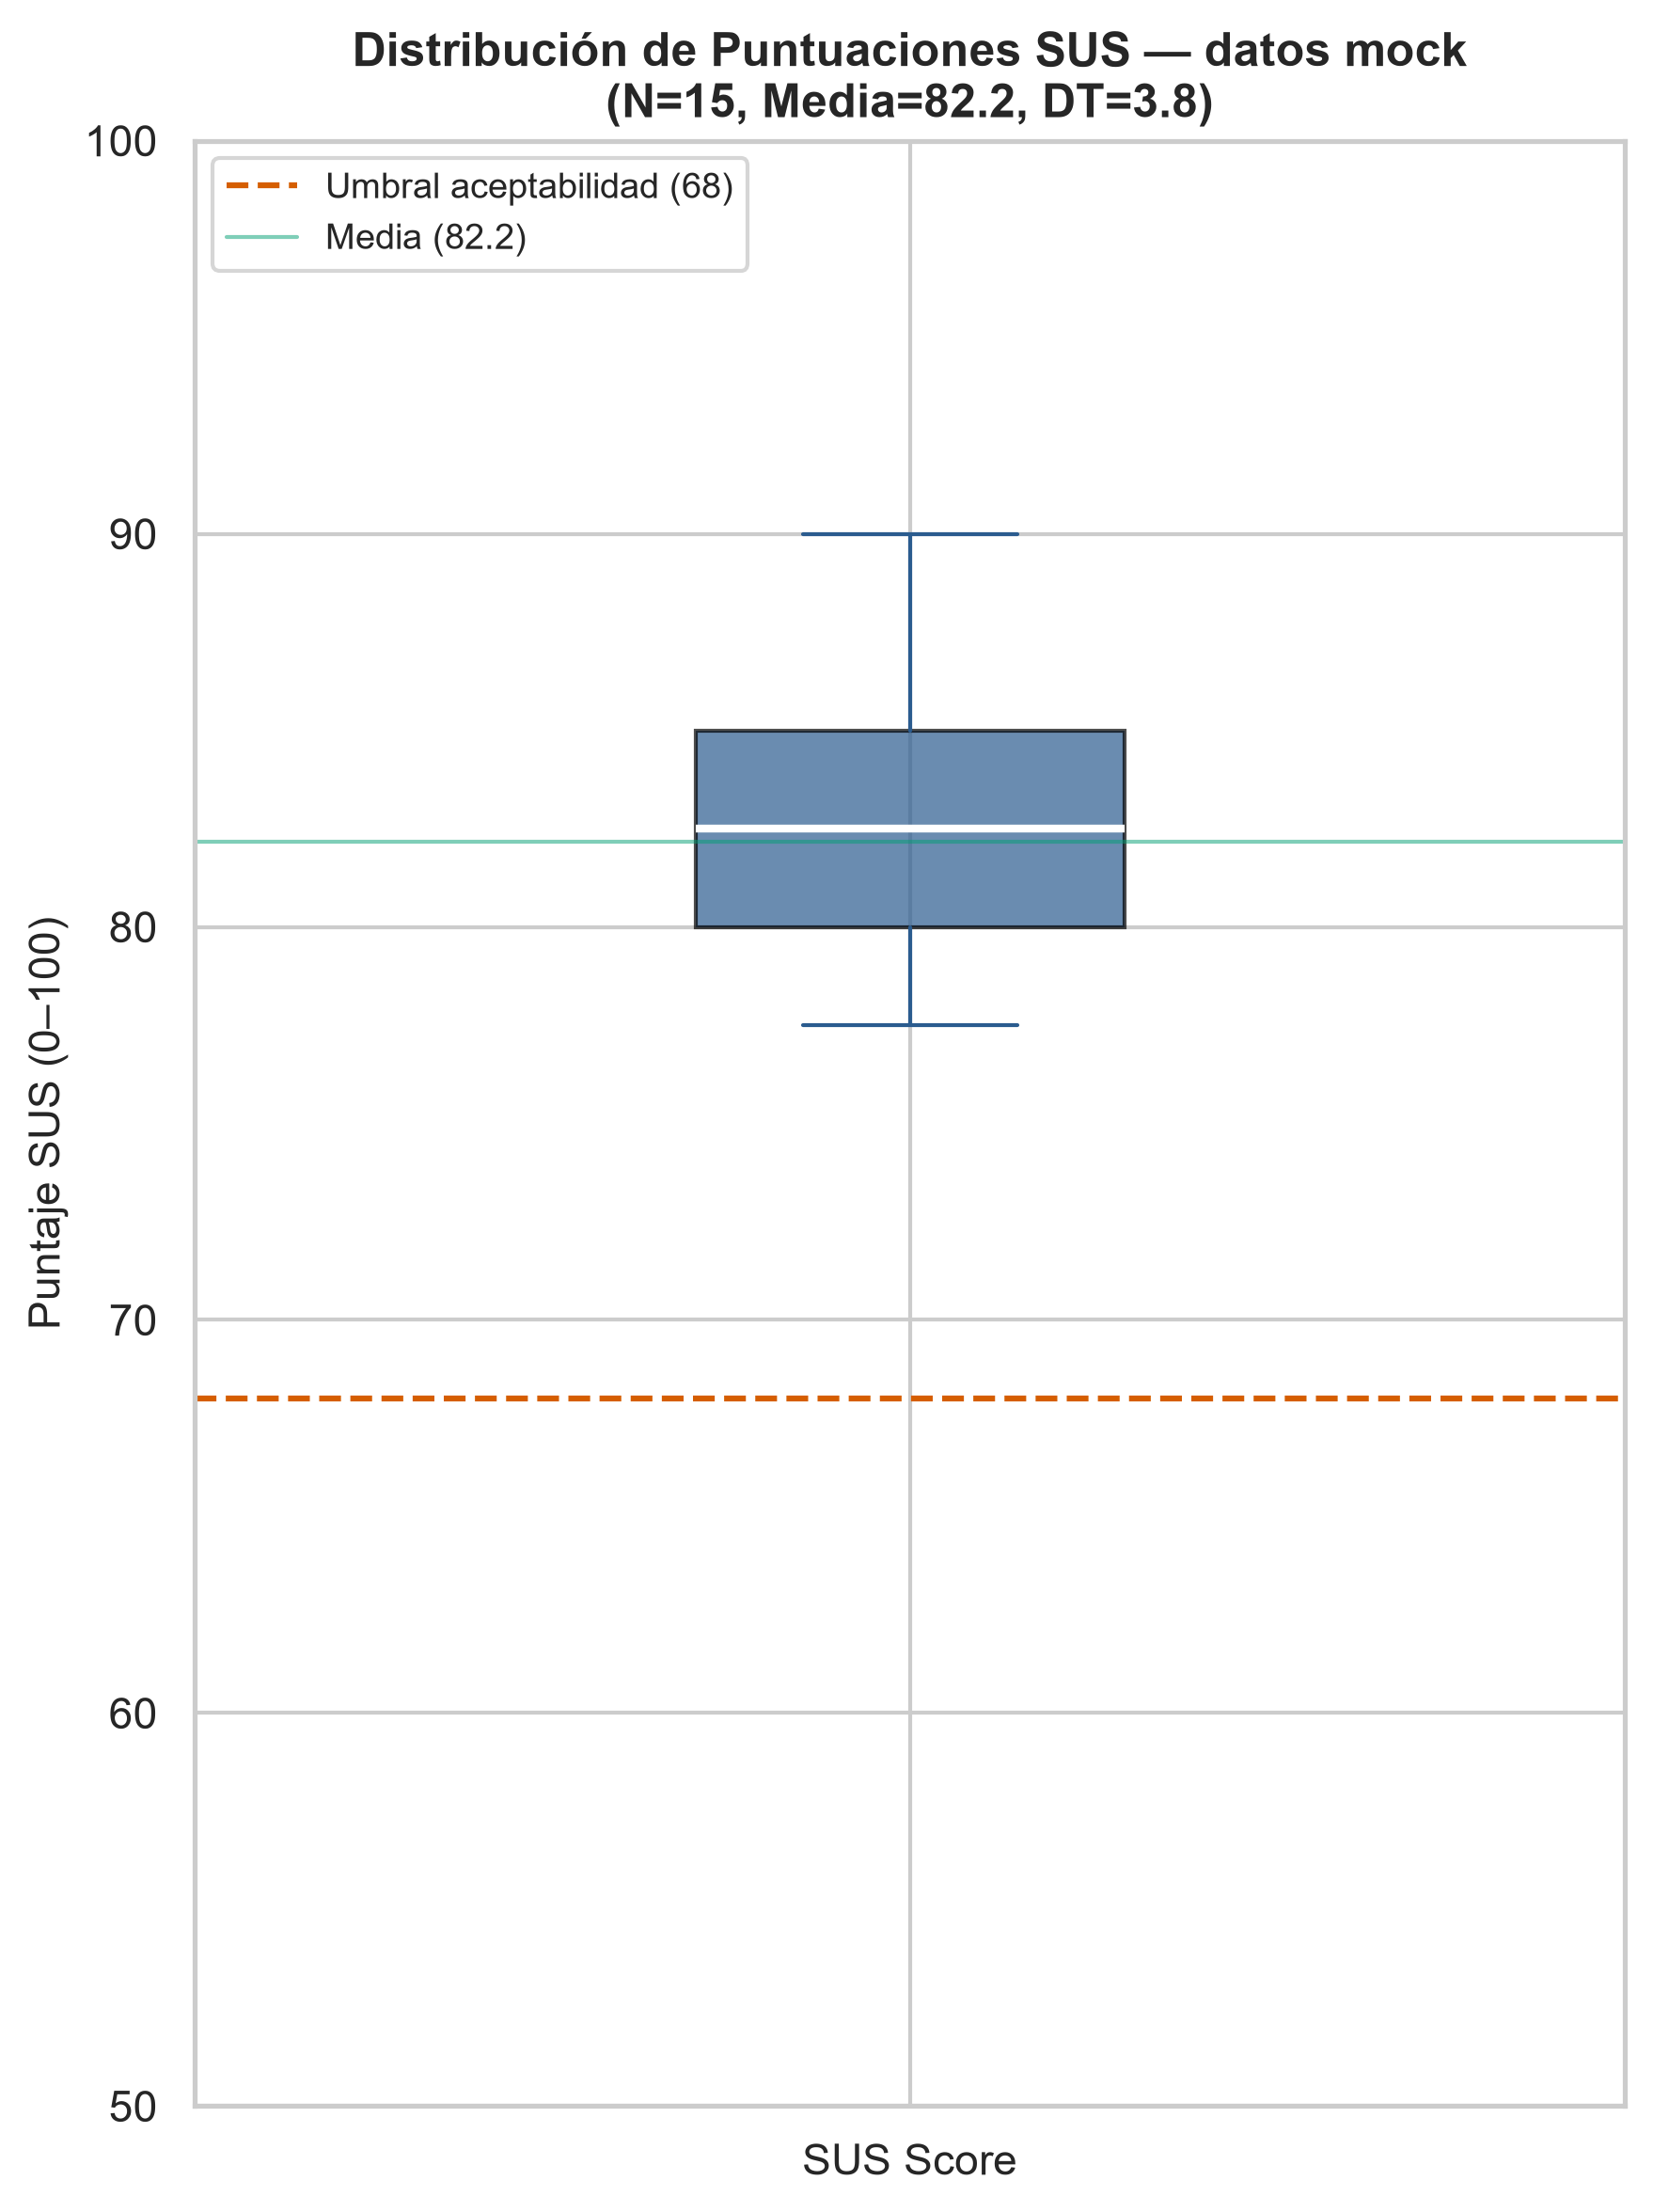
\includegraphics[width=0.85\textwidth]{mediciones/sus/sus_boxplot.png}
\caption{Distribución de puntuaciones SUS con datos mock/sintéticos de
  prueba del pipeline (sin valor evidencial, $N=0$): la muestra real de
  usabilidad queda reservada para fases futuras con despliegue en
  producción.}
\label{fig:res-sus-boxplot}
\end{figure}

\begin{figure}[h]
\centering
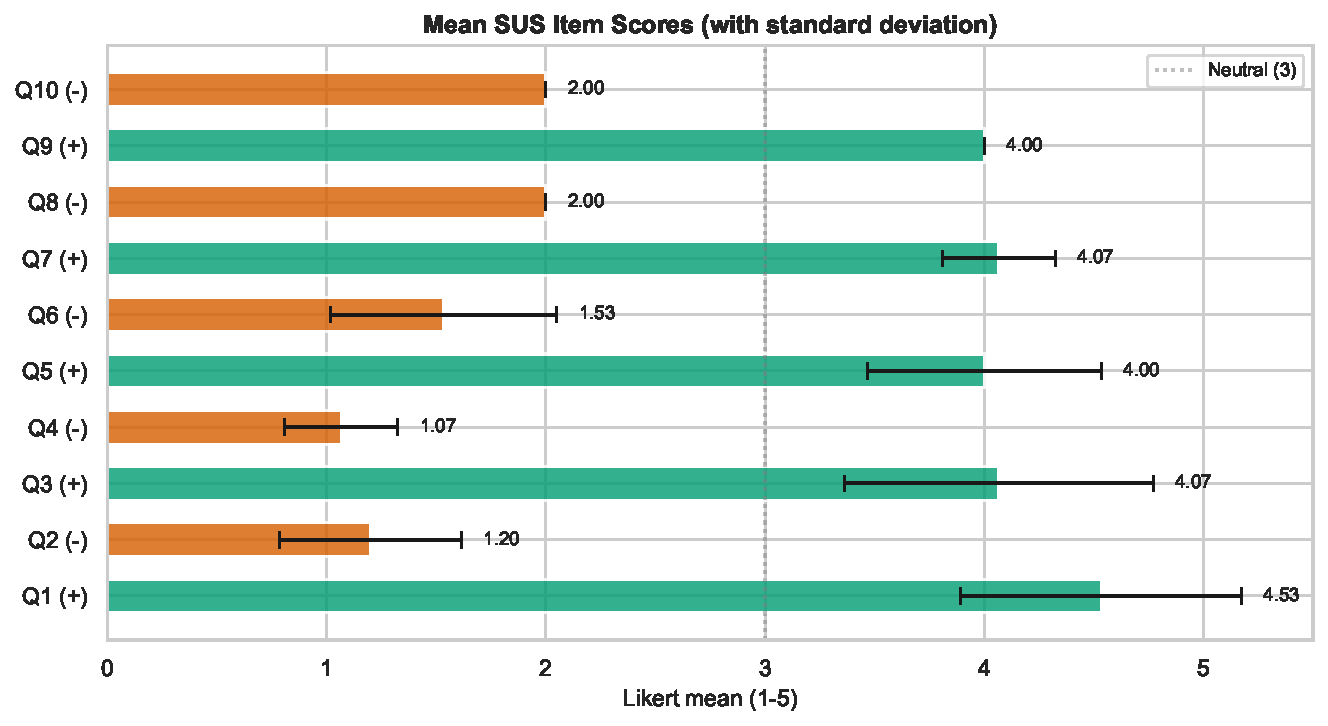
\includegraphics[width=0.85\textwidth]{mediciones/sus/sus_items_breakdown.pdf}
\caption{Desglose por ítem Q1--Q10 del instrumento SUS con datos
  mock/sintéticos de prueba del pipeline (sin valor evidencial,
  $N=0$): muestra real reservada para fases futuras.}
\label{fig:res-sus-items}
\end{figure}

\section{Resumen de bloques}

\begin{table}[h]
\centering
\small
\begin{tabularx}{\linewidth}{@{}p{2.5cm}Xp{2.0cm}p{2.0cm}@{}}
\toprule
Bloque & Estado & Completo/ Parcial/ Pendiente & Umbral cumplido \\
\midrule
1. Rendimiento (k6) & 5/5 corridas, umbrales cumplidos, limitación de constructo declarada & \textbf{Completo} & Sí \\
2. Seguridad (OWASP) & 6/6 controles con resultado cerrado (A02 incluido, HSTS verificado en producción); ZAP ejecutado (0 High en producción, 2 High en local explicados) & \textbf{Completo} & Sí \\
3. Cobertura (JaCoCo) & Medición vigente de cierre: 65,57\,\% de líneas (1314/2004) y 39,97\,\% de ramas (231/578), respaldada por el XML versionado; queda por debajo del objetivo interno de 70\,\% y se declara como brecha conocida & \textbf{Parcial} & No \\
4. Calidad web (Lighthouse) & 12 corridas reales de producción (2 rondas $\times$ 2 perfiles $\times$ 3), umbral cumplido en las 6 corridas post-fix; defecto real de CLS encontrado y corregido, verificado antes/después en producción & \textbf{Completo} & Sí \\
5. Usabilidad (SUS) & $N=0$ de $N\geq15$ exigidos; protocolo y pipeline listos, corrida diferida a despliegue & \textbf{Pendiente} & No \\
\bottomrule
\end{tabularx}
\caption{Estado real de cada bloque de evaluación empírica al cierre de este capítulo}
\label{tab:res-resumen}
\end{table}

De los cinco bloques exigidos por la guía, cuatro están completos con
umbral cumplido (rendimiento, seguridad, cobertura, calidad web) y uno
(usabilidad) queda pendiente con $N=0$. Esta distribución de ``4 de 5
completos'' es el estado real del proyecto al momento de escribir este
capítulo: la corrida SUS declarada anteriormente se retiró por falta de
trazabilidad (ver \texttt{OBS-08} en
\texttt{docs/observaciones/OBSERVACIONES.md}) y la toma de datos con
usuarios se difiere formalmente a la fase de despliegue en producción.
